% Żeby nie było syfu to kolejne sekcje dodajemy do chapters/
% A potem includujemy za pomocą \input{chapters/...}

% Używamy \( \) i \[ \] zamiast dolarów -- tak jak się robi w LaTeXu


\documentclass[12pt, a4paper, polish, openany]{book}

% Please, let's familiarize ourselves with notatki.sty and tcs.sty so that we don't reinvent the wheel
\usepackage{notatki}
\fancyhead[L]{\textbf{\textit{MPI}}}

\begin{document}
% Front page and table of contents
\frontmatter

\begin{titlepage}

	\begin{center}
		\begin{figure}[h]
			\centering
			\includegraphics[scale=0.75]{img/bumblebee.jpg}
		\end{figure}
		\vspace{0.5cm}
		\Huge
		\textbf{\textsc{Metody Probabilistyczne Informatyki - Opracowanie pytań egzaminacyjnych}}

		\normalsize

		\line(1,0){330}

		\vspace{1cm}
		
		\textit{,,Co dalej? Boże... co dalej? Co my w ogóle robimy tutaj? Nie wiem.''}
		\vspace{1cm}

		\textit{\textsc{Popełnione przez}}\\
		\vspace{5mm}

		\textbf{\textsc{
				Załatany Ponton \\
				V\\
				Nahtamatu\\
			}}
			% TODO: dodać autorów
		\vfill

		Kraków \\
		Anno Domini 2025

	\end{center}

\end{titlepage}


\tableofcontents
\input{license}

% Remove the "Rozdział x" chapter headings, as we already number our chapters
\titleformat{\chapter}[display]{\normalfont\Huge\bfseries}{}{0pt}{\Huge}
\titlespacing*{\chapter}{0pt}{0pt}{20pt}

\newenvironment{questiontext}
    {
     \vspace{1em}
     \begin{center}
     \begin{minipage}{0.9\textwidth}
     \fontsize{14}{14}\selectfont
     \setlength{\parskip}{1em}
    }
    {
     \end{minipage}
     \end{center}
     \vspace{2em}
     \hrule height 0.5pt
     \vspace{2em}
    }

% Actual content
\mainmatter

\chapter{Pytanie 1}
{
\makeatletter
\def\input@path{{../probabil}}
\makeatother
\graphicspath{{../probabil}}

\begin{questiontext}
    Rozkład dwumianowy, rozkład geometryczny i ich własności. Własność bez pamięci, wartość oczekiwana, wariancja, wyższe momenty. Funkcje tworzące momentów.
\end{questiontext}

\section{Rozkład dwumianowy}
{
	\ExecuteMetaData[chapters/discrete-probability/binomial]{probabil-egzamin-rozklad-dwumianowy-1}
	\ExecuteMetaData[chapters/discrete-probability/binomial]{probabil-egzamin-rozklad-dwumianowy-2}
	\ExecuteMetaData[chapters/discrete-probability/binomial]{probabil-egzamin-rozklad-dwumianowy-3}
}

\section{Rozkład geometryczny}
{
	\ExecuteMetaData[chapters/discrete-probability/geometric]{probabil-egzamin-rozklad-geometryczny-1}
	\ExecuteMetaData[chapters/discrete-probability/geometric]{probabil-egzamin-rozklad-geometryczny-2}
	W oparciu na funkcję tworzącą momenty, możemy obliczyć wartość oczekiwaną, wariancję, oraz dowolne wyższe momenty
	\ExecuteMetaData[chapters/discrete-probability/geometric]{probabil-egzamin-rozklad-geometryczny-3}
}

}

\chapter{Pytanie 2}
{
\makeatletter
\def\input@path{{../probabil}}
\makeatother
\graphicspath{{../probabil}}

\begin{questiontext}
    Problem kolekcjonera kuponów (wartość oczekiwana). Oczekiwana liczba porównań w algorytmie sortowania Quicksort.
\end{questiontext}

{
	\let\realsection\section
	\let\realsubsection\subsection
	\let\subsection\section
	\let\subsubsection\paragraph

	\ExecuteMetaData[chapters/discrete-probability/expected-value-problems]{probabil-egzamin-kolekcjoner-kuponow}
	\ExecuteMetaData[chapters/discrete-probability/expected-value-problems]{probabil-egzamin-quicksort}
}
}

\chapter{Pytanie 3}
{
\makeatletter
\def\input@path{{../probabil}}
\makeatother
\graphicspath{{../probabil}}

\begin{questiontext}
    Własności wariancji. Nierówność Markowa. Nierówność Czebyszewa i jej zastosowanie w problemie kolekcjonera kuponów.
\end{questiontext}

\section{Wariancja}
{
	\ExecuteMetaData[chapters/discrete-probability/variance]{probabil-egzamin-wariancja}
}

\section{Nierówność Markowa}
{
	\ExecuteMetaData[chapters/inequalities/markov]{probabil-egzamin-markov}
}

\section{Nierówność Czebyszewa}
{
	\subsection{Definicja}
	\ExecuteMetaData[chapters/inequalities/chebyshev]{probabil-egzamin-chebyshev-1}
	\ExecuteMetaData[chapters/inequalities/chebyshev]{probabil-egzamin-chebyshev-2}
}
}

\chapter{Pytanie 4}
{
\makeatletter
\def\input@path{{../probabil}}
\makeatother
\graphicspath{{../probabil}}

\begin{questiontext}
    Ogólny schemat nierówności Czernowa. Nierówność Czernowa dla sum niezależnych prób Poissona. Zastosowanie tej nierówności: niezależne rzuty sprawiedliwą monetą.
\end{questiontext}

\section{Nierówność Czernowa}
{
	\ExecuteMetaData[chapters/inequalities/chernoff]{probabil-egzamin-chernoff-1}
	\ExecuteMetaData[chapters/inequalities/chernoff]{probabil-egzamin-chernoff-2}
	\ExecuteMetaData[chapters/inequalities/chernoff]{probabil-egzamin-chernoff-3}
}
}

\chapter{Pytanie 5}
{
\makeatletter
\def\input@path{{../probabil}}
\makeatother
\graphicspath{{../probabil}}

\begin{questiontext}
    Kule i urny: obciążenie najcięższej urny prawie zawsze jest co najwyżej \(\frac{3 \ln n}{\ln \ln n}\).
\end{questiontext}

\section{Kule i urny - ograniczenie górne}
\input{chapters/discrete-probability/balls-and-bins}
}

\chapter{Pytanie 6}
{
\makeatletter
\def\input@path{{../probabil}}
\makeatother
\graphicspath{{../probabil}}

\begin{questiontext}
    Rozkład Poissona i jego własności: momenty, suma niezależnych zmiennych, tworząca momentów i ograniczenia Chernowa.
\end{questiontext}

\section{Rozkład Poissona}
\subsection{Podstawowe własności}
\begin{definition}
	\textbf{Stochastycznym procesem liczącym} nazywamy \hyperref[stochastic-process-definition]{proces stochastyczny} 
	\[\set{N(t) \mid t \geq 0}\] 
	
	spełniający
	\begin{enumerate}
		\item \(N(t) \in \natural_0\)
		\item \(\forall_{s < t} N(s) \leq N(t)\)
	\end{enumerate}
\end{definition}

Intuicyjnie: \(N(t)\) mówi ile \textit{jakichś} zdarzeń zaszło od momentu rozpoczęcia procesu do chwili \(t\), a dla \(s \leq t\) liczba zdarzeń które zaszły w przedziale czasu \((s, t]\) to \(N(t) - N(s)\).

\begin{definition}
	\label{poisson-process-definition}
	\textbf{Procesem Poissona} z parametrem \( \lambda \) nazywamy stochastyczny proces liczący \( \set{N(t) \mid t \in \real, t \geq 0} \) taki, że:

	\begin{enumerate}
		\item \( N(0) = 0 \)
		
		\item Proces ma stacjonarne i niezależne przyrosty, tzn.
		\begin{enumerate}[label=\arabic{enumi}\alph*.]
			\item Stacjonarność: \(\forall_{s, t \geq 0}\) zmienne \(N(s)\) oraz \(N(s+t) - N(t)\) mają taki sam rozkład
			\item Niezależność: \(\forall_{t_1 < t_2 \leq t_3 < t_4}\) zmienne \( N(t_2) - N(t_1) \) oraz \( N(t_4) - N(t_3) \) są niezależne
		\end{enumerate}
		
		\item Prawdopodobieństwo jednego zdarzenia w małym przedziale długości \( t \) zbiega do \( \lambda  \) \\
		      \[ \lim_{t \rightarrow 0} \frac{\prob(N(t) = 1)}{t} = \lambda \]

		\item Prawdopodobieństwo więcej niż jednego zdarzenia w małym przedziale zbiega do zera \\
		      \[ \lim_{t \rightarrow 0} \frac{\prob(N(t) > 1)}{t} = 0 \]
	\end{enumerate}
\end{definition}


\subsection{Ograniczenia Czernowa}
\input{chapters/poisson-distribution/chernoff-bounds}
}

\chapter{Pytanie 7}
{
\makeatletter
\def\input@path{{../probabil}}
\makeatother
\graphicspath{{../probabil}}

\begin{questiontext}
    Aproksymacja Poissona oraz jej zastosowanie do problemu kul i urn: obciążenie najcięższej urny jest prawie zawsze co najmniej \(\frac{\ln n}{\ln \ln n}\).
\end{questiontext}

\section{Aproksymacja Poissona}
{
	\ExecuteMetaData[chapters/poisson-distribution/poisson-approximation]{probabil-egzamin-aproksymacja-poissona}
}
}

\chapter{Pytanie 8}
{
\makeatletter
\def\input@path{{../probabil}}
\makeatother
\graphicspath{{../probabil}}

\begin{questiontext}
    Problem kolekcjonera kuponów: granica prawdopodobieństwa, że nie zbierzemy wszystkich \(n\) kuponów po \(n \ln n + cn\) krokach.
\end{questiontext}
}

\chapter{Pytanie 9}
{
\makeatletter
\def\input@path{{../probabil}}
\makeatother
\graphicspath{{../probabil}}

\begin{questiontext}
    Łańcuch Markowa. Nieprzywiedlność, okres stanu i okres łańcucha. Okres nieprzywiedlnego łańcucha Markowa. Własność nieprzywiedlnego i nieokresowego łańcucha Markowa. Stany powracające (dodatnie i zerowe) i chwilowe. W każdym nieprzywiedlnym, skończonym łańcuchu Markowa oczekiwany czas przejścia pomiędzy dwoma stanami jest skończony.
\end{questiontext}
}

\chapter{Pytanie 10}
{
\makeatletter
\def\input@path{{../probabil}}
\makeatother
\graphicspath{{../probabil}}

\begin{questiontext}
    Rozkład stacjonarny. Istnienie, unikalność oraz interpretacja.
\end{questiontext}

\section{Rozkład stacjonarny}
{
	\ExecuteMetaData[chapters/markov-chains/definitions]{probabil-egzamin-10-rozklad-stacjonarny}
}
}

\chapter{Pytanie 11}
{
\makeatletter
\def\input@path{{../probabil}}
\makeatother
\graphicspath{{../probabil}}

\begin{questiontext}
    Norma całkowitego wahania rozkładów prawdopodobieństwa, własności normy, sprzęganie rozkładów prawdopodobieństwa. Związek między normą a sprzęganiem
\end{questiontext}

\section{Norma całkowitego wahania}
{
	\ExecuteMetaData[chapters/coupling/distributions]{probabil-egzamin-11-norma-calkowitego-wahania}
}

\section{Sprzęganie rozkładów prawdopodobieństwa}
{
	\ExecuteMetaData[chapters/coupling/distributions]{probabil-egzamin-11-sprzeganie}
}
}

\chapter{Pytanie 12}
{
\makeatletter
\def\input@path{{../probabil}}
\makeatother
\graphicspath{{../probabil}}

\begin{questiontext}
    Lemat o sprzęganiu łańcuchów Markowa, lemat o monotoniczności.
\end{questiontext}
}

\chapter{Pytanie 13}
{
\makeatletter
\def\input@path{{../probabil}}
\makeatother
\graphicspath{{../probabil}}

\begin{questiontext}
    Twierdzenie o geometrycznej zbieżności rozkładu stanu łańcucha do rozkładu stacjonarnego.
\end{questiontext}
}

\chapter{Pytanie 14}
{
\makeatletter
\def\input@path{{../probabil}}
\makeatother
\graphicspath{{../probabil}}

\begin{questiontext}
    Losowe spacery w grafie jako zastosowanie łańcuchów Markowa.
\end{questiontext}
}

\chapter{Pytanie 15}
{
\makeatletter
\def\input@path{{../probabil}}
\makeatother
\graphicspath{{../probabil}}

\begin{questiontext}
    Rozkład jednostajny: gęstość, dystrybuanta, momenty, funkcja tworząca momentów, rozkład pod warunkiem, że wylosowano wartość poniżej ustalonego progu, wartość oczekiwana \(k\)-tej statystyki \(n\) niezależnych prób zmiennych o rozkładzie jednostajnym.
\end{questiontext}

\section{Rozkład jednostajny}
{
    \ExecuteMetaData[chapters/continuous-probability/uniform]{probabil-egzamin-15-rozklad-jednostajny}	
}
}

\chapter{Pytanie 16}
{
\makeatletter
\def\input@path{{../probabil}}
\makeatother
\graphicspath{{../probabil}}

\begin{questiontext}
    Rozkład wykładniczy. Gęstość, dystrybuanta, momenty, funkcja tworząca momentów, własność bez pamięci, rozkład minimum \(n\) niezależnych prób. Funkcja Gamma i rozkład Gamma. Związek z rozkładem wykładniczym.
\end{questiontext}

\section{Rozkład wykładniczy}
{	
	\ExecuteMetaData[chapters/continuous-probability/exponential]{probabil-egzamin-16-rozklad-wykladniczy-1}
	\ExecuteMetaData[chapters/continuous-probability/exponential]{probabil-egzamin-16-rozklad-wykladniczy-2}
}

\section{Funkcja Gamma i rozkład Gamma}
{
	\ExecuteMetaData[chapters/continuous-probability/gamma]{probabil-egzamin-16-gamma-1}
	\ExecuteMetaData[chapters/continuous-probability/gamma]{probabil-egzamin-16-gamma-2}
}
}

\chapter{Pytanie 17}
{
\makeatletter
\def\input@path{{../probabil}}
\makeatother
\graphicspath{{../probabil}}

\begin{questiontext}
    (8.3.2). Problem kul i urn ze wzmocnionym feedbackiem.
\end{questiontext}

\section{Kule i urny z feedbackiem}
{	
	\ExecuteMetaData[chapters/continuous-probability/exponential]{probabil-egzamin-17-kule-urny-feedback}
}
}

\chapter{Pytanie 18}
{
\makeatletter
\def\input@path{{../probabil}}
\makeatother
\graphicspath{{../probabil}}

\begin{questiontext}
    (8.4). Proces Poissona. Definicja. Prawdopodobieństwo pojawienia się \(n\) zdarzeń w ustalonym odcinku czasowym długości \(t\) (Twierdzenia 8.7 i 8.8).
\end{questiontext}
}

\chapter{Pytanie 19}
{
\makeatletter
\def\input@path{{../probabil}}
\makeatother
\graphicspath{{../probabil}}

\begin{questiontext}
    (8.4.1). Proces Poissona. Rozkład czasów pomiędzy zdarzeniami (Twierdzenia 8.9, 8.10 i 8.11).
\end{questiontext}
}

\chapter{Pytanie 20}
{
\makeatletter
\def\input@path{{../probabil}}
\makeatother
\graphicspath{{../probabil}}

\begin{questiontext}
    (8.4.2). Scalanie i rozdzielanie procesów Poissona (Twierdzenia 8.12 i 8.13).
\end{questiontext}

\section{Scalanie i rozdzielanie procesów Poissona}
\input{chapters/poisson-process/splitting-and-merging}
}

\chapter{Pytanie 21}
{
\makeatletter
\def\input@path{{../probabil}}
\makeatother
\graphicspath{{../probabil}}

\begin{questiontext}
    (8.4.3). Warunkowe czasy pojawiania się zdarzeń w procesie Poissona (Twierdzenie 8.14).
\end{questiontext}
\input{chapters/poisson-process/conditional-arrival-times}
}

\chapter{Pytanie 22}
{
\makeatletter
\def\input@path{{../probabil}}
\makeatother
\graphicspath{{../probabil}}

\begin{questiontext}
    Naturalny proces losowy motywujący gęstość rozkładu normalnego. Rozkład normalny. Własności. Funkcja tworząca.
\end{questiontext}

\section{Standardowy rozkład normalny}
\subsection{Wyprowadzenie}
Rozważmy sobie rozkład na \(\real^2\) o następujących własnościach:
\begin{itemize}
	\item gęstość wokół każdego punktu zależy jedynie od odległości od środka układu (w szczególności rotacja nie zmienia rozkładu).
	\item wartości współrzędnych \(x\) i \(y\) są od siebie niezależne.
	\item ten rozkład jest ciągły.
\end{itemize}

Okazuje się, że istnieje tylko jeden taki rozkład (z dokładnością do stałej), nazywamy go standardowym rozkładem normalnym. Oznaczamy go przez \( Z \sim N(0,1) \).

Zgodnie z definicją, gęstość zależy jedynie od odległości punktu od środka układu współrzędnych. Możemy więc to zapisać jako:
    \[
    f((x, y)) = f(r) = f\pars{\sqrt{x^2 + y^2}} = g(x)h(y) = g(x)g(y)
    \]
Ostatnie przekształcenie wynika z tego, że nasza gęstość nie zależy od rotacji, więc możemy obrócić wszystko o \(90\) stopni.
Dodatkowo, dla punktu \((r, 0 )\) równanie przyjmie postać:
    \[
    f((r, 0)) = g(r)g(0)
    \]
gdzie \( g(0) \) jest stałą. Z tego powodu możemy wstępnie założyć, że \( f = g \) a potem całość odpowiednio przeskalować. Tak więc teraz mamy:
    \[
    f\pars{\sqrt{x^2 + y^2}} = f(x)f(y)
    \]
Niech:
    \[ 
    h(x) = f\pars{\sqrt{x}} 
    \]
Wtedy:
    \[ h(x^2) = f(x) \]
    \[ h(x^2 + y^2) = h(x^2)h(y^2) \]
    \[ h(x + y) = h(x)h(y) \]

Z ostatniego punktu można przez indkucję pokazać, że \( \forall_{n \in \natural} \forall_{x_1, \ldots, x_n \in \real} h(x_1 + \ldots + x_n) = h(x_1)\ldots h(x_n) \)
Niech \( h(1) = b \). Korzystając z poprzedniego faktu mamy, że \(\forall_{n \in \natural} h(n) = b^n \).

Teraz chcemy udowodnić to samo dla liczb wymiernych:
    \[
    h\pars{\frac{p}{q} + \ldots + \frac{p}{q}} = h(p) = b^p = h\pars{\frac{p}{q}}^q
    \]
Gdzie na początku mamy dokładnie \(q\) ułamków \( \frac{p}{q} \) w funkcji \(h\).
Przekształcając ostatnią równość otrzymujemy:
    \[
    h\pars{\frac{p}{q}} = b^{\frac{p}{q}}
    \]

Na koniec chcemy udowodnić to samo dla liczb rzeczywistych (co na wykładzie chyba pominęliśmy).
Z MFI pamiętamy, że każdą liczbę rzeczywistą możemy przybliżyć jakimś ciągiem liczb wymiernych, a bardziej formalnie:
    \[
    \forall_{x \in \real} \exists_{q_n} x = \lim_{n \to \infty} q_n
    \]
Gdzie \( q_n \) jest jakimś ciągiem liczb wymiernym. Z połączenia tego faktu i założenia o ciągłości funkcji \(h\) otrzymamy:
    \[
    h(x) = h\pars{\lim_{n \to \infty} q_n} = \lim_{n \to \infty}h(q_n) = \lim_{n \to \infty} b^{q_n} = b^{\lim_{n \to \infty} q_n} = b^x
    \]

Ustalmy:
    \[
    	b = e^c \implies h(x) = e^{cx}
    \]

Teraz podstawiamy to do naszej funkcji gęstości, uwzględniamy skalowanie i otrzymujemy:
    \[
    f(z) = a \cdot e^{cx^2}
    \]
Gdzie \( c < 0 \). \\


Przyjmijmy \( c = -\frac{1}{2} \). Teraz chcemy znaleźć stałą \( a \). Oczywiście chcemy, żeby pole pod naszą funkcją wynosiło 1, więc wystarczy obliczyć odpowiednią całkę.
Całki:
    \[
    \int_{-\infty}^{\infty} e^{-\frac{z^2}{2}} \diff z 
    \]
nie jesteśmy w stanie ładnie rozwiązać, więc posłużymy się takim trikiem:
    \begin{align*}
    \int_{-\infty}^{\infty} e^{-\frac{z^2}{2}} \diff z \cdot \int_{-\infty}^{\infty} e^{-\frac{z^2}{2}} \diff z &= \int_{-\infty}^{\infty} \int_{-\infty}^{\infty} e^{-\frac{x^2 + y^2}{2}} \diff x \diff y \\
    &= \int_0^{2\pi} \int_0^{\infty} e^{-\frac{r^2}{2}} \cdot e \diff r \diff \theta \\
    &= \int_0^{2\pi} \int_0^{\infty} e^{-u} \diff u \diff \theta \\
    &= \int_0^{2\pi} 1 \diff \theta = 2\pi
    \end{align*}
Gdzie kolejno druga i trzecia równość to przejście na współrzędne biegunowe, oraz podstawienie \( u = \frac{r^2}{2} \) (dlatego przyjęliśmy akurat \( c = -\frac{1}{2} \) ).
Dalej mamy:
    \[
    \int_{-\infty}^{\infty} e^{-\frac{z^2}{2}} \diff z = \sqrt{2\pi} \implies a = \frac{1}{\sqrt{2\pi}}
    \]

\begin{minipage}[c]{0.5\linewidth}
	\[
		f(z) = \frac{1}{\sqrt{2\pi}} e^{-\frac{z^2}{2}}
	\]
\end{minipage}
\quad
\begin{minipage}[c]{0.4\linewidth}
	\centering
	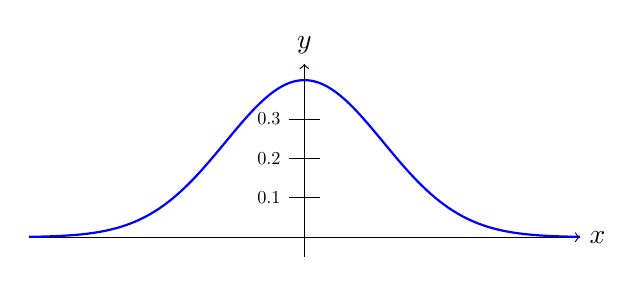
\begin{tikzpicture}
	\draw[->] (-3.5, 0) -- (3.5, 0) node[right] {$x$};
	\draw[->] (0, -0.25) -- (0, 2.2) node[above] {$y$};
	\draw[domain=-3.5:3.5, samples=100, yscale=5, smooth, variable=\x, blue, thick] plot ({\x}, {1/sqrt(2*pi) * exp(-0.5*\x*\x)});
	\draw (-0.2,0.5) -- (0.2,0.5);
	\node[scale=0.66] at (-0.45,0.5) {\(0.1\)};
	\draw (-0.2,1) -- (0.2,1);
	\node[scale=0.66] at (-0.45,1) {\(0.2\)};
	\draw (-0.2,1.5) -- (0.2,1.5);
	\node[scale=0.66] at (-0.45,1.5) {\(0.3\)};
\end{tikzpicture}
\end{minipage}

Funkcja gęstości prawdopodobieństwa standardowego rozkładu normalnego wygląda jak \sout{dzban} dzwon.


\subsection{Właściwości}
\begin{theorem}
	Wartość oczekiwana standardowego rozkładu normalnego wynosi 0, wariancja wynosi 1.
\end{theorem}

\begin{proof}
	Wartość oczekiwana wynosi 0, ponieważ standardowy rozkład normalny jest symetryczny wobec prostej \( OY\)
	Wariancja:
	\[
		\variance{Z} = \expected{Z^2} - \expected{Z}^2 = \expected{Z^2} = \\
	\]
	ponieważ \( \expected{Z} = 0 \)
	\[
		= \frac{1}{\sqrt{2\pi}}\int_{-\infty}^{z}t^2e^{-t^2/2} dt =
	\]
	\[
		= \frac{1}{\sqrt{2\pi}}\int_{-\infty}^{z}(t)(te^{-t^2/2}) dt =
	\]
	całkowanie przez części
	\[
		\brackets{-\frac{1}{\sqrt{2\pi}}te^{-t^2/2}}_{-\infty}^{\infty} + \frac{1}{\sqrt{2\pi}}\int_{-\infty}^{\infty}e^{-t^2/2} dt = 1
	\]
	Ponieważ pierwszy wyraz jest równy 0 a drugi jest to dystrybuanta na od \(-\infty \) do \( \infty \) więc wynosi ona 1.
\end{proof}
\begin{definition}
	Dystrybuantę standardowego rozkładu normalnego oznaczamy jako \( \Phi \), gdzie:
	\[
		\Phi(z) = \frac{1}{\sqrt{2\pi}} \int_{-\infty}^{z} e^{-\frac{t^2}{2}} \diff t
	\]
	Oraz:
	\[
		\Phi(-z) = 1 - \Phi(z)
	\]
	Ta całka generalnie nie jest do policzenia, jeżeli trzeba skorzystać z dystrybuanty to są do tego specjalne tabele wartości
\end{definition}


\section{Uogólniony rozkład normalny}
\begin{definition}
	Dla \(Z \sim N(0, 1)\) definiujemy (uogólniony) rozkład normalny \(X \sim N(\mu, \sigma^2)\) jako
	\[
		X = \mu + \sigma Z
	\]
\end{definition}

\begin{theorem}
	Dla \(X \sim N(\mu, \sigma^2)\) zachodzi
	\begin{itemize}
		\item \(\ev{X} = \mu\)
		\item \(\variance{X} = \sigma^2\)
		\item \(F_X(x) = \Phi(\frac{x - \mu}{\sigma})\)
		\item \(f_X(x) = \frac{1}{\sigma \sqrt{2\pi}}e^{-\frac{\pars{x-\mu}^2}{2\sigma^2}}\)
	\end{itemize}
\end{theorem}
\begin{proof}
	Ponieważ zmienna losowa \( X\) z \(N(\mu, \sigma^2) \) ma ten sam rozkład co \( \mu + \sigma Z \) mamy że
	\[
		\expected{X} = \expected{\mu + \sigma Z} = \mu + \sigma \ev{Z} = \mu
	\]
	\[
		\variance{X} = \variance{\sigma Z + \mu} = \sigma^2 \variance{Z} = \sigma^2
	\]
	\[
		F_X(x) = \prob\pars{X \leq x} = \prob\pars{\frac{X-\mu}{\sigma} \leq \frac{x-\mu}{\sigma}} = \prob\pars{Z \leq \frac{x-\mu}{\sigma}} = \Phi\pars{\frac{x-\mu}{\sigma}}
	\]
	\[
		f_X(x) = (F_X(x))' = \pars{\Phi\pars{\frac{x-\mu}{\sigma}}}' = \frac{1}{\sigma} \pars{\frac{1}{\sqrt{2\pi}} \int_{-\infty}^{x} e^{-\frac{\pars{\frac{t-\mu}{\sigma}}^2}{2}} \diff t}' = \frac{1}{\sigma \sqrt{2\pi}}e^{-\frac{\pars{x-\mu}^2}{2\sigma^2}}
	\]
\end{proof}

\begin{theorem}
	Funkcja tworząca momemty rozkładu normalnego \(N(\mu, \sigma^2)\) wynosi
	\[
		\mathcal{M}_X(t) = e^{\frac{t^2\sigma^2}{2}+\mu t}
	\]
\end{theorem}
\begin{proof}
	\begin{align*}
		\mathcal{M}_X(t) &= \mathbb{E}[e^{tX}] \\
		&= \frac{1}{\sqrt{2\pi}\sigma}\int_{-\infty}^{\infty} e^{tx} e^{-\frac{(x-\mu)^2}{2\sigma^2}} dx \\
		&= \frac{1}{\sqrt{2\pi}\sigma}\int_{-\infty}^{\infty} \exp\left( -\frac{x^2 - 2\mu x + \mu^2 - 2\sigma^2 tx}{2\sigma^2} \right) dx \\
		&= \frac{1}{\sqrt{2\pi}\sigma}\int_{-\infty}^{\infty} \exp\left( -\frac{x^2 - 2(\mu + \sigma^2 t)x + (\mu + \sigma^2 t)^2 - (\mu + \sigma^2 t)^2 + \mu^2}{2\sigma^2} \right) dx \\
		&= \exp\left( \frac{(\mu + \sigma^2 t)^2 - \mu^2}{2\sigma^2} \right) \underbrace{\int_{-\infty}^{\infty} \frac{1}{\sqrt{2\pi}\sigma} e^{-\frac{(x - (\mu + \sigma^2 t))^2}{2\sigma^2}} dx}_{1} \\
		&= \exp\left( \frac{\mu^2 + 2\mu\sigma^2 t + \sigma^4 t^2 - \mu^2}{2\sigma^2} \right) \\
		&= e^{\mu t + \frac{t^2\sigma^2}{2}}
	\end{align*}
	
	Całka w 3 linii od dołu jest równa 1, bo jest to całka po gęstości rozkładu \(N(\mu + \sigma^2 t, \sigma^2)\).
\end{proof}

\begin{theorem}
	Niech \(X \sim N(\mu_1, \sigma^2_1), Y \sim N(\mu_2, \sigma^2_2)\) to niezależne zmienne losowe. Wtedy \(X+Y \sim N(\mu_1+\mu_2, \sigma_1^2+\sigma_2^2)\).
\end{theorem}
\begin{proof}
	\begin{align*}
		\mathcal{M}_{X+Y}(t) = \pars{\mathcal{M}_X(t)}\pars{\mathcal{M}_Y(t)} = \pars{e^{\frac{t^2\sigma_1^2}{2}+\mu_1 t}}\pars{e^{\frac{t^2\sigma_2^2}{2}+\mu_2 t}} =\\
		= e^{\frac{t^2(\sigma_1^2+\sigma_2^2)}{2} + t(\mu_1 + \mu_2)}
	\end{align*}
\end{proof}

Podobnie możemy pokazać, że dla niezależnych \(X_1 \sim N(0, \sigma_1^2), X_2 \sim N(0, \sigma_2^2)\) dostajemy \(X_1+X_2 \sim N(0, \sigma_1^2+\sigma_2^2)\) oraz \(X_1-X_2 \sim N(0, \sigma_1^2+\sigma_2^2)\).

}

\chapter{Pytanie 23}
{
\makeatletter
\def\input@path{{../probabil}}
\makeatother
\graphicspath{{../probabil}}

\begin{questiontext}
    (9.3). Centralne Twierdzenie Graniczne. Dowód. Warianty mocniejszych wypowiedzi.
\end{questiontext}

\section{Centralne Twierdzenie Graniczne}
%<*probabil-2025-12-19-centralne-twierdzenie-graniczne-1>
\subsection{Podstawowa wersja}
Intuicyjnie: Centralne Twierdzenie Graniczne mówi, że jak mamy niezależne zmienne losowe o takim samym rozkładzie, to dla liczby prób zbiegającej do nieskończoności rozkład średniej arytmetycznej tych wylosowanych wartości będzie zbiegać do rozkładu normalnego.
Twierdzenie to uzasadnia występowanie w naturze rozkładu normalnego.
%</probabil-2025-12-19-centralne-twierdzenie-graniczne-1>
\begin{definition}
	Ciąg dystrybuant \( F_1, F_2, ... \) zbiega w dystrybuancie do dystrybuanty \( F\), co oznaczamy jako \(F_n \to F \), jeśli dla każdego \(a \in \mathbb{R} \) w którym \( F \) jest ciągła zachodzi:
	\[
		\lim_{n \to \infty} F_n(a) = F(a)
	\]
\end{definition}

%<*probabil-2025-12-19-centralne-twierdzenie-graniczne-2>
\begin{theorem}[Centralne Twierdzenie Graniczne]
	Niech \(\set{X_i}_{i \in \natural}\) będą niezależnymi zmiennymi losowymi o takim samym rozkładzie, wartości oczekiwanej \( \mu\) i wariancji \( \sigma^2\). Niech \( \widetilde{X_n} = \frac{1}{n}\sum_{i=1}^n X_i \). Wówczas dla dowolnych \(a, b\)
	\[
		\lim_{n \to \infty} \prob \pars{a \leq \frac{ \widetilde{X_n} - \ev{\widetilde{X_n}}}{\sqrt{\variance{\widetilde{X_n}}}} \leq b} = \Phi(b) - \Phi(a)
	\]
\end{theorem}
\begin{proof}
	Pierwsze, przekształćmy sobie trochę nasz cel
	\[
		\ev{\widetilde{X_n}} = \mu
	\]
	\[
		\variance{\widetilde{X_n}} = \variance{\frac{1}{n}\sum_{i=1}^n X_i} = \frac{1}{n^2} \variance{\sum_{i=1}^n X_i} = \frac{1}{n^2} \sum_{i=1}^n \variance{X_i} = \frac{1}{n^2} n \sigma^2 = \frac{\sigma^2}{n}
	\]
	A więc
	\[
		\lim_{n \to \infty} \prob \pars{a \leq \frac{ \widetilde{X_n} - \ev{\widetilde{X_n}}}{\sqrt{\variance{\widetilde{X_n}}}} \leq b} = \lim_{n \to \infty} \prob \pars{a \leq \frac{ \widetilde{X_n} - \mu}{\sigma} \cdot \sqrt{n} \leq b}
	\]
	
	Dalej, aby dowieść CTG, będziemy musieli przytoczyć \textit{pomocne twierdzonko}, którego (mamy nadzieję) nikt nie będzie musiał dowodzić:

	\begin{theorem}[Lévy-Cramér] 
		Niech \(\set{Y_i}_{i \in \natural}\) będzie sekwencją zmiennych losowych, gdzie \(Y_i\) ma dystrybuantę \(F_i\) i funkcję tworzącą momenty \( M_i\). Niech \(Y\) będzie zmienną losową o dystrybuancie \(F\) i funkcji tworzącej momenty \(M\). Jeżeli dla każdego \(t\) zachodzi:
		\[
			\lim_{n \to \infty}M_n(t) = M(t)
		\]

		to dla każdego \(t\) takiego, że \(F\) jest ciągła w \(t\) zachodzi
		\[
			\lim_{n \to \infty} F_n(t) = F(t)
		\]
	\end{theorem}
	\begin{proof}
		Mitzenmacher przytacza to twierdzenie bez dowodu; na wykładzie go również nie było, a więc i my udowodnimy je poprzez założenie go jako aksjomat (haha).
	\end{proof}

	Przystępujemy teraz do dowodzenia CTG.

	Definiujemy \( Z_i = \frac{X_i - \mu}{\sigma} \).
	Wówczas \( Z_i\) są niezależnymi zmiennymi losowymi oraz

	\[
		\expected{Z_i} = \expected{\frac{X_i - \mu}{ \sigma}} = \frac{1}{\sigma} \cdot \pars{\expected{X_i} - \expected{\mu}} = \frac{1}{\sigma} \cdot \pars{\mu - \mu} = 0
	\]

	\[
		\variance{Z_i} = \variance{\frac{X_i - \mu}{\sigma}} = \frac{1}{\sigma^2} \cdot \pars{\variance{X_i - \mu}} = \frac{1}{\sigma^2} \cdot \pars{\variance{X_i} - \variance{\mu}} = \frac{1}{\sigma^2} \cdot \pars{\sigma^2 - 0} = 1
	\]
	
	\[
		\variance{Z_i} = \ev{Z_i^2} - \ev{Z_i}^2 \implies \ev{Z_i^2} = \variance{Z_i} + \ev{Z_i}^2 = 1 + 0^2 = 1
	\]

	Ponadto mamy, że:
	\[
		\frac{\widetilde{X_n} - \mu}{\sigma} \cdot \sqrt{n} 
		= \frac{\sum_{i=1}^n \frac{X_i}{n} - \mu}{\sigma} \cdot \sqrt{n} 
		= \frac{\sum_{i=1}^n \frac{X_i - \mu}{n}}{\sigma} \cdot \sqrt{n} 
		= \frac{\sqrt{n}}{n}\sum_{i=1}^{n}\frac{X_i-\mu}{\sigma} 
		= \frac{\sum_{i=1}^nZ_i}{\sqrt{n}}
	\]
	Żeby zastosować teraz przywołane przez nas twierdzenie Levy'ego i tego drugiego musimy pokazać, że funkcja tworząca momenty zmiennych losowych postaci
	\[
		Y_n = \frac{\sum_{i=1}^nZ_i}{\sqrt{n}}
	\]
	zbiega do funkcji tworzącej momenty zmiennej losowej o standardowym rozkładzie normalnym. Po zastosowaniu tego twierdzenia dostalibyśmy już tezę Centralnego Twierdzenia Granicznego.

	W takim razie, chcemy pokazać
	\[
		\lim_{n \to \infty} M_{Y_n}(t) = \lim_{n \to \infty}\expected{e^{t\frac{\sum_{i=1}^nZ_i}{\sqrt{n}}}} = e^{\frac{t^2}{2}}
	\]
	Niech \( M_{Z_i}(t) = \expected{e^{tZ_i}} \) będzie funkcją tworzącą momenty zmiennej \(Z_i\).  Zauważamy, że wówczas funkcja tworząca momenty zmiennej losowej \( \frac{Z_i}{\sqrt{n}}\) wynosi
	\[
		M_{\frac{Z_i}{\sqrt{n}}} (t) = \expected{e^{t \cdot \frac{Z_i}{\sqrt{n}}}} = M_{Z_i} \pars{\frac{t}{\sqrt{n}}}
	\]
	Ponieważ \( Z_i\) są niezależne i mają ten sam rozkład mamy
	\[
		M_{Y_n}(t) = M_{\sum_{i=1}^{n} \frac{Z_i}{\sqrt{n}}} (t) = \pars{M_{\frac{Z_i}{\sqrt{n}}}(t)}^n = \pars{M_{Z_i}\pars{\frac{t}{\sqrt{n}}}}^n
	\]

	Teraz wykonujemy \textit{magiczne założenie}. Zdefiniujmy sobie, \textbf{for no reason at all}, funkcję \(L\), taką że

	\[
		L(t) = \ln M_{Z_i}(t)
	\]

	Dodatkowo, \textit{również bez jakiejkolwiek przyczyny}, policzmy sobie pierwszą i drugą pochodną \(L(0)\).

	Zacznijmy od trywialnych obserwacji:
	\[
		M_{Z_i}(0) = 1 \implies L(0) = 0
	\]
	\[
		L'(0) = \pars{\ln M_{Z_i}(0)}' = \frac{1}{M_{Z_i}(0)} \cdot M'_{Z_i}(0) = \frac{M_{Z_i}'(0)}{M_{Z_i}(0)} = \frac{\expected{Z_i}}{1} = \expected{Z_i} = 0
	\]
	\[
		L''(0) = \frac{M_{Z_i}(0)M_{Z_i}''(0) - (M_{Z_i}'(0))^2}{(M_{Z_i}(0))^2} = \frac{M_{Z_i}''(0) - 0}{1} = \expected{Z_i^2} = 1
	\]

	Przypomnijmy, że chcieliśmy pokazać, że


	\[
		\lim_{n\to\infty}M_{Y_n}\pars{t} = \lim_{n \to \infty } \pars{M_{Z_i}\pars{\frac{t}{\sqrt{n}}}}^n = e^{\frac{t^2}{2}}
	\]
	
	po zlogarytmowaniu stronami

	\[
		\lim_{n \to \infty} nL\pars{\frac{t}{\sqrt{n}}} = \frac{t^2}{2}
	\]

	Pytanie teraz co musimy zrobić by wykazać, że ta granica tyle wynosi.

	Jak wszyscy wiemy, kiedy nie wiadomo jak policzyć granicę, to liczymy ją L’Hôpitalem. Zapiszmy więc sobie ten limit tak, byśmy mogli użyć tego twierdzenia (czyli żeby pojawił się symbol nieoznaczony \( \frac{0}{0} \)).
	\[
		\lim_{n \to \infty}\frac{L\pars{\frac{t}{\sqrt{n}}}}{n^{-1}}
	\]

	No i lecimy z pochodnymi!

	\begin{align*}
		\lim_{n \to \infty}\frac{L \pars{\frac{t}{\sqrt{n}}}}{n^{-1}} &= \brackets{\frac{0}{0}}\\
		&= \lim_{n \to \infty}\frac{-\frac{1}{2}L'\pars{\frac{t}{\sqrt{n}}}tn^{-\frac{3}{2}}}{-n^{-2}}               \\
		& = \lim_{n \to \infty}\frac{L'\pars{\frac{t}{\sqrt{n}}}t}{2n^{-\frac{1}{2}}}                       \\
		&= \brackets{\frac{0}{0}}\\
		& = \lim_{n \to \infty}\frac{-\frac{1}{2}L''\pars{\frac{t}{\sqrt{n}}}t^2 n^{-\frac{3}{2}}}{-\frac{1}{2}2n^{-\frac{3}{2}}} \\
		& = \lim_{n \to \infty} \frac{t^2 \cdot L''\pars{\frac{t}{\sqrt{n}}}}{2}                            \\
		& = \lim_{n \to \infty} \frac{t^2 \cdot 1 }{2}                                                      \\
		& = \frac{t^2}{2}
	\end{align*}

	I w sumie to mieliśmy dowieść. Ale fajnie.
\end{proof}

\subsection{Warianty}
Istnieją różne warianty CTG, które mają swoje zastosowania w różnych sytuacjach. Poniżej podajemy wypowiedzi dwóch takich wariantów.

W pierwszym wariancie usuwamy warunek na to, że wszystkie zmienne \(X_i\) muszą mieć taki sam rozkład, ale musimy za to dodać dwa dodatkowe warunki.
\begin{theorem}
	Niech \(\set{X_i}_{i \in \natural}\) będzie ciągiem niezależnych zmiennych losowych spełniających \(\mathbb{E}\left[ X_i \right] = \mu_i\) i \(\variance{X_i} = \sigma_i^2\). Niech zachodzi
	\begin{enumerate}
		\item \(\exists_{M>0} \ \forall_{i \in \natural} \ P\left( \left|X_i\right|<M \right) = 1 \)
		\item \( \lim_{n \to \infty} \sum_{i=1}^{n} \sigma_i^2 = +\infty\).
	\end{enumerate}
	Wówczas dla dowolnych \(a, b\) zachodzi
	\[ 
		\lim_{n \to \infty} P\left( a \le \frac{ \sum_{i=1}^{n} \left( X_i - \mu_i \right) }{\sqrt{ \sum_{i=1}^{n} \sigma_i^2} } \le  b  \right) = \Phi\pars{b} - \Phi\pars{a}
	\]
\end{theorem}

Za to w drugim wariancie mając dodakową informację o trzecim momencie, możemy wyznaczyć prędkość zbiegania do rozkładu normalnego
\begin{theorem}[Berry-Ess\'een]
	Istnieje taka stała \(C\), że dla każdego ciągu niezależnych zmiennych losowych \(\set{X_i}_{i \in \natural}\) o tym samym rozkładzie ze skończoną wartością oczekiwaną \(\mu\) i wariancją \(\sigma^2\) oraz dla \(\rho = \mathbb{E}\left[ \left|X_i-\mu\right|^3 \right] < \infty \) i \(\widetilde{X_n} = \frac{1}{n} \sum_{i=1}^{n} X_i\) zachodzi
	
	\[ 
		\left|P\left( \frac{\widetilde{X_n}-\mu}{\frac{\sigma}{\sqrt{n} }} \le a \right) - \Phi\left( a  \right) \right| \le C\cdot \frac{\rho}{\sigma^3 \sqrt{n} }
	\]
\end{theorem}
%</probabil-2025-12-19-centralne-twierdzenie-graniczne-2>
}

\chapter{Wprowadzenie siły dwóch wyborów}
{
\makeatletter
\def\input@path{{../probabil}}
\makeatother
\graphicspath{{../probabil}}

\label{two-choices-introduction}
Pytania 24-26 wszystkie są związane z siłą dwóch wyborów i wymagają wypowiedzi tych samych twierdzeń oraz modelu eksperymentu. Dodatkowo, częściowo używają tych samych oznaczeń oraz lematów. Aby uniknąć powtarzania tych segmentów, są one wszystkie obecne tutaj.

{
	\let\realsection\section
	\let\realsubsection\subsection
	\let\subsection\section
	\let\subsubsection\paragraph
	\subsection{Wprowadzenie modelu eksperymentu}
W tej sekcji wracamy do znanego nam już problemu kul i urn. W \ref{balls-and-bins-max-load-upper-bound} oraz \ref{balls-and-bins-max-load-lower-bound} pokazaliśmy, że jeśli dla wystarczająco dużego \(n\) wrzucamy \(n\) kul do \(n\) urn niezależnie i jednostajnie oraz \(X_i\) to liczba kul w \(i\)-tej urnie, to
\[
	\prob\pars{\frac{\ln n}{\ln \ln n} \leq \max(X_1, \dots, X_n) \leq 3\frac{\ln n}{\ln \ln n}} \geq 1 - \frac{2}{n}
\]
Na wykładzie było powiedziane, że jest to prawda nie tylko dla \(\frac{2}{n}\), ale dla \(\frac{1}{n^\alpha}\) dla dowolnego \(\alpha\), ale nie było na to żadnego dowodu, a więc raczej nie trzeba tego wiedzieć.

Rozważmy teraz wariant standardowego eksperymentu z kulami i urnami. %
%<*probabil-egzamin-24-26-introduction-1>
Rzucamy \(n\) kul sekwencyjnie do \(n\) urn i dla każdej kuli symulujemy dwa rzuty. Kula trafia do tej urny z dwóch wylosowanych która jest mniej wypełniona, a remisy rozsrzygamy dowolnie. Okazuje się, że znacząco zmienia to rozkład \(\max(X_1, \dots, X_n)\), co pokazuje następujące twierdzenie

\begin{theorem}
	\label{power-of-two-choices-theorem}
	W opisanym powyżej modelu \(\forall_{\alpha \geq 1} \, \exists_{n_0} \, \forall_{n \geq n_0}\) zachodzi
	\[
		\prob\pars{\frac{\ln \ln n}{\ln 2} - \mathcal{O}_\alpha(1) \leq \max(X_1, \dots, X_n) \leq \frac{\ln \ln n}{\ln 2} + \mathcal{O}_\alpha(1)} \geq 1 - \frac{1}{n^\alpha}
	\]
	lub równoważnie
	\[
		\prob\pars{\log_2 \ln n - \mathcal{O}_\alpha(1) \leq \max(X_1, \dots, X_n) \leq \log_2 \ln n + \mathcal{O}_\alpha(1)} \geq 1 - \frac{1}{n^\alpha}
	\]
\end{theorem}
Dodatkowo, jeśli symulujemy \(d\) rzutów zamiast dwóch, w powyższym wzorze zamiast \(\ln 2\) jest obecne \(\ln d\) i musimy zamienić \(\mathcal{O}_\alpha(1)\) na jakieś \(\mathcal{O}_{d, \alpha}(1)\). Widzimy, że nie zmienia to bardzo naszych ograniczeń, a dowody tych wariantów są bardzo podobne, a więc dla uproszczenia nasze rozumowanie będziemy przeprowadzać dla \(d = 2\).
%</probabil-egzamin-24-26-introduction-1>

Dla demonstracji tego, o ile lepsze jest losowanie z dwoma symulacjami od standardowego eksperymentu, możemy użyć \href{https://medium.com/the-intuition-project/load-balancing-the-intuition-behind-the-power-of-two-random-choices-6de2e139ac2f}{artykułu}, którego autor przeprowadził symulację komputerową wrzucenia miliona kul do tysiąca urn. Histogram po lewej pokazuje rozkład liczby kul w urnie dla losowego przydzielenia urn, a histogram po prawej dla wyboru lepszej urny z dwóch.
\includegraphics[width=\linewidth]{img/power-of-two-choices/simulated-distributions.png}

%<*probabil-egzamin-24-26-introduction-2>
\subsection{Lematy pomocnicze}
\begin{lemma}
	\label{chernow-for-power-of-two}
	Dla \(Z \sim \Bin(n, p)\) zachodzi
	\[
		\prob(Z \geq 2np) \leq e^{-\frac{np}{3}}
	\]
	\[
		\prob\pars{Z \leq \frac{1}{2}np} \leq e^{-\frac{np}{8}}
	\]
\end{lemma}
\begin{proof}
	Pierwsza nierównośc wynika wprost z punktu 2. \ref{poisson-trial-chernoff-bounds} z \(\delta = 1\), a druga z punktu 2. \ref{poisson-trial-chernoff-lowerbounds} z \(\delta = \frac{1}{2}\).
	\[
		\ev{Z} = np
	\]
	\[
		\prob(Z \geq 2np) = \prob(Z \geq (1 + \delta)\ev{Z}) \leq e^{-\frac{1}{3} \ev{Z} \delta^2} = e^{-\frac{np}{3}}
	\]
	\[
		\prob\pars{Z \leq \frac{1}{2}np} = \prob(Z \leq (1 - \delta)\ev{Z}) \leq e^{-\frac{1}{2} \ev{Z} \delta^2} = e^{-\frac{np}{8}}
	\]
\end{proof}

\begin{lemma}
	\label{binary-random-variable-binomial-upperbound}
	Niech \(X_1, \dots, X_n\) to zmienne losowe, \(Y_1, \dots, Y_n\) to binarne zmienne losowe, \(Y_i = f_i(X_1, \dots, X_i)\) (jest wyznaczona przez \(X_1, \dots, X_i\)) oraz \(Z \sim \Bin(n, p)\) jest niezależna od poprzednich zmiennych. Jeśli dla każdego \(i \in [n]\) oraz \((x_1, \dots, x_{i - 1})\) takiego, że \(\prob((X_1, \dots, X_{i - 1}) = (x_1, \dots, x_{i - 1})) > 0\) zachodzi
	\[
		\prob(Y_i = 1 \mid (X_1, \dots, X_{i - 1}) = (x_1, \dots, x_{i - 1})) \leq p
	\]
	to
	\[
		\prob\pars{\sum_{i = 1}^n Y_i > k} \leq \prob(Z > k)
	\]
\end{lemma}
\begin{proof} (dla \(n = 3\), dla wyższych \(n\) analogicznie)
	\begin{align*}
		\prob(Y_1 + Y_2 + Y_3 > k) &\leq \prob(Z_1 + Y_2 + Y_3 > k) \\
		&= \sum\nolimits_{x_1} \prob(Z_1 + Y_2 + Y_3 > k \mid X_1 = x_1) \cdot \prob(X_1 = x_1) \\
		&\leq \sum\nolimits_{x_1} \prob(Z_1 + Z_2 + Y_3 > k \mid X_1 = x_1) \cdot \prob(X_1 = x_1) \\
		&= \sum\nolimits_{(x_1, x_2)} \prob(Z_1 + Z_2 + Y_3 > k \mid (X_1, X_2) = (x_1, x_2)) \\
		&\qquad\qquad\quad \cdot \prob(X_2 = x_2 \mid X_1 = x_1) \cdot \prob(X_1 = x_1) \\
		&\leq \sum\nolimits_{(x_1, x_2)} \prob(Z_1 + Z_2 + Z_3 > k \mid (X_1, X_2) = (x_1, x_2)) \\
		&\qquad\qquad\quad \cdot \prob(X_2 = x_2 \mid X_1 = x_1) \cdot \prob(X_1 = x_1) \\
		&= \sum\nolimits_{(x_1, x_2)} \prob(Z_1 + Z_2 + Z_3 > k) \\
		&\qquad\qquad\quad \cdot \prob(X_2 = x_2 \mid X_1 = x_1) \cdot \prob(X_1 = x_1) \\
		&= \prob(Z_1 + Z_2 + Z_3 > k) \cdot \sum\nolimits_{(x_1, x_2)} \prob(X_2 = x_2 \mid X_1 = x_1) \prob(X_1 = x_1) \\
		&= \prob(Z_1 + Z_2 + Z_3 > k)
	\end{align*}
\end{proof}

\begin{lemma} (Lemat dualny dla \ref{binary-random-variable-binomial-upperbound}) 
	\label{binary-random-variable-binomial-lowerbound}
	Niech \(X_1, \dots, X_n\) to zmienne losowe, \(Y_1, \dots, Y_n\) to binarne zmienne losowe, \(Y_i = f_i(X_1, \dots, X_i)\) (jest wyznaczona przez \(X_1, \dots, X_i\)) oraz \(Z \sim \Bin(n, p)\) jest niezależna od poprzednich zmiennych. Jeśli dla każdego \(i \in [n]\) oraz \((x_1, \dots, x_{i - 1})\) takiego, że \(\prob((X_1, \dots, X_{i - 1}) = (x_1, \dots, x_{i - 1})) > 0\) zachodzi
	\[
		\prob(Y_i = 1 \mid (X_1, \dots, X_{i - 1}) = (x_1, \dots, x_{i - 1})) \geq p
	\]
	to
	\[
		\prob\pars{\sum_{i = 1}^n Y_i > k} \geq \prob(Z > k)
	\]
	a więc też
	\[
		\prob\pars{\sum_{i = 1}^n Y_i < k} \leq \prob(Z < k)
	\]
\end{lemma}
\begin{proof}
	Tak samo jak w poprzednim lemacie.
\end{proof}

\subsection{Oznaczenia}
Do dowodów ograniczenia górnego przez iterację ograniczeń oraz ograniczenia dolnego przydadzą nam się funkcje pomocnicze. Dla \(t \in [n]\) niech
\begin{itemize}
	\item \(h(t)\) to wysokość \(t\)-tej kuli, czyli liczba kul w urnie, w której wylądowała \(t\)-ta kula zaraz po jej wrzuceniu
	\item \(\nu_i(t)\) to liczba urn zawierających \(\geq i\) kul zaraz po wrzuceniu \(t\)-tej kuli
	\item \(\mu_i(t)\) to liczba kul o wysokości \(\geq i\) zaraz po wrzuceniu \(t\)-tej kuli
\end{itemize}

Prosto widzimy, że 
\[
	\forall_{i \in [n], \, t \in [n]} \,\, \nu_i(t) \leq \mu_i(t)
\]
bo w każdej urnie zawierającej \(\geq i\) kul jest przynajmniej jedna kula wysokości \(\geq i\). 
%</probabil-egzamin-24-26-introduction-2>

}
}

\chapter{Pytanie 24}
{
\makeatletter
\def\input@path{{../probabil}}
\makeatother
\graphicspath{{../probabil}}

\begin{questiontext}
    Siła dwu wyborów. Model eksperymentu, wypowiedzi twierdzeń. Dowód ograniczenia górnego (ten w książce) przez iterację ograniczeń na prawdopodobieństwa warunkowe pewnych zdarzeń.
\end{questiontext}

W tej sekcji znajduje się wyłącznie dowód ograniczenia górnego górnego przez iterację ograniczeń na prawdopodobieństwa warunkowe. Model eksperymentu oraz wypowiedzi twierdzeń znajdują się w rozdziale \ref{two-choices-introduction}.

\section{Ograniczenie górne przez iterację ograniczeń}
Przejdźmy wreszcie do pierwszego dowodu ograniczenia górnego twierdzenia \ref{power-of-two-choices-theorem}. Niech
\[
	\beta_4 = \frac{n}{4}
\]
\[
	\beta_{i+1} = 2\frac{\beta_i^2}{n} \text{ dla } 4 \leq i \leq i^*
\]
\(i^*\) zostanie zdefiniowane później.

\begin{lemma}
	\[
		\beta_{i+4} = \frac{n}{2^{2^i + 1}}
	\]
	a więc
	\[
		\beta_{i+4} \leq \frac{n}{2^{2^i}}
	\]
\end{lemma}
\begin{proof}
	Przeprowadźmy dowód indukcyjny. Dla \(i = 0\)
	\[
		\beta_4 = \frac{n}{4} = \frac{n}{2^{1 + 1}} = \frac{n}{2^{2^0 + 1}} = \beta_{0 + 4}
	\]
	Jeśli lemat zachodzi dla \(i\) to
	\[
		\beta_{i+5} = 2\frac{\beta_{i+4}^2}{n} 
		= 2\frac{\pars{\frac{n}{2^{2^i + 1}}}^2}{n} 
		= 2\frac{n}{2^{2(2^i + 1)}}
		= 2\frac{n}{2^{2^{i + 1} + 2}}
		= \frac{n}{2^{2^{i + 1} + 1}}
		= \beta_{(i + 1) + 4}
	\]
	a więc zachodzi też dla \(i + 1\)
\end{proof}

Zdefiniujmy teraz \(\mathcal{E}_i\) jako zdarzenie zachodzące jeśli \(\nu_i(n) \leq \beta_i\). Widzimy, że
\[
	\prob(\mathcal{E}_4) = \prob\pars{\nu_4(n) \leq \frac{n}{4}} = 1
\]
bo oczywiście \(\geq \frac{n}{4}\) kul może mieć co najwyżej \(\frac{n}{4}\) urn.

Chcemy teraz wykazać, że jeśli \(\mathcal{E}_i\) zaszło, to prawie na pewno \(\mathcal{E}_{i + 1}\) też zaszło. Dla \(t \in [n]\) definiujemy binarną zmienną losową \(Y_t\)
\[
	Y_t = \left\{ \begin{array}{lr} 1 & \text{ dla } h(t) \geq i + 1 \land \nu_i(t - 1) \leq \beta_i \\ 0 & \text{wpp.} \end{array} \right.
\]
Zauważmy, że dla \((K_1, \dots, K_{t - 1})\) będącego zmiennymi losowymi reprezentującymi urny do których trafiły kolejne kule oraz \((\omega_1, \dots, \omega_{t - 1})\) takiego, że \(\forall_{i \in [t - 1]} \, \omega_i \in [n]\) zachodzi
\[
	\prob(Y_t = 1 \mid (K_1, \dots, K_{t - 1}) = (\omega_1, \dots, \omega_{t - 1})) \leq \pars{\frac{\beta_i}{n}}^2
\]
Jest tak, ponieważ aby zaszło \(h(t) \geq i + 1\) \(t\)-ta kula musi obiema symulacjami trafić w urnę o przynajmniej \(i\) kulach, ale wiemy z \(\nu_i(t - 1) \leq \beta_i \) że takich urn jest co najwyżej \(\beta_i\) z \(n\) możliwych.

Jeśli \(\mathcal{E}_i\) zaszło, to \(\mu_{i+1}(n) = \sum_{t \in [n]} Y_t\), ponieważ z \(\mathcal{E}_i\) wiemy, że \(\nu_i(t - 1) \leq \beta_i\) jest prawdziwe dla każdego \(t\), a więc \(Y_t = 1 \iff h(t) \geq i + 1\), a więc suma \(Y_t\) zlicza liczbę kul o wysokości \(\geq i + 1\), co jest dokładnie definicją \(\mu_{i+1}(n)\).

Niech \(p_i \coloneq \pars{\frac{\beta_i}{n}}^2\). Z lematu \ref{binary-random-variable-binomial} dostajemy
\[
	\prob\pars{\sum_{t \in [n]} Y_t > k} \leq \prob(\Bin(n, p_i) > k)
\]
}

\chapter{Pytanie 25}
{
\makeatletter
\def\input@path{{../probabil}}
\makeatother
\graphicspath{{../probabil}}

\begin{questiontext}
    (\(\star\)). Siła dwu wyborów. Model eksperymentu, wypowiedzi twierdzeń. Dowód ograniczenia górnego przez drzewa świadczące.
\end{questiontext}

W tej sekcji znajduje się wyłącznie dowód ograniczenia górnego przez drzewa świadczące. Model eksperymentu oraz wypowiedzi twierdzeń znajdują się w rozdziale \ref{two-choices-introduction}.

\section{Ograniczenie górne przez drzewa świadczące}
Poniższy dowód wzorowany jest artykułem \href{https://dl.acm.org/doi/10.1145/792538.792546}{\textit{How asymmetry helps load balancing}}.

\subsection*{Definicje drzew świadczących}

Jak poprzednio, rzucając kulę losujemy jednostajnie \(d \geq 2\) urn i wrzucamy kulę do najmniej wypełnionej. Będziemy dalej nazywać \(i\)-tą wylosowaną urnę dla kuli \(b\) \(i\)-tą lokacją kuli \(b\).

\begin{definition}
    \textbf{Drzewo świadczące} rzędu \(L\) to pełne, ukorzenione drzewo \(d\)-arne wysokości \(L\).
    Każdy wierzchołek w drzewie reprezentuje pewną kulę, niekoniecznie unikalną - kula może być reprezentowana przez wiele wierzchołków.
    Dodatkowo, dla każdego wierzchołka \(v\) niebędącego liściem, kule odpowiadające dzieciom \(v\) muszą już znajdować się w urnach w momencie rzucania kuli \(v\).
\end{definition}

Ogólna idea dowodu będzie następująca; rozważmy wszystkie drzewa świadczące.
Powiemy za moment, co oznacza, że dla danego rzucenia kul do urn konkretne drzewo świadczące jest \textit{aktywne}, a następnie pokażemy, że jeśli w którejś z urn jest dużo kul, to istnieje \textit{aktywne} drzewo świadczące odpowiedniego rzędu.
Tym samym prawdopodobieństwo, że któraś urna ma dużo kul jest ograniczone przez prawdopodobieństwo, że istnieje odpowiednie \textit{aktywne} drzewo świadczące.

\begin{definition}
    Dodajmy sobie dodatkową intepretację dla struktury dowolnego drzewa świadczącego.

    \begin{itemize}
        \item \textbf{Krawędziozdarzenie} (\textit{"edge event"}) - dla krawędzi \(e = \pars{u, v}\), gdzie \(v\) jest \(i\)-tym dzieckiem \(u\),
        krawędź \(e\) określa zdarzenie, że \(i\)-ta lokacja kuli \(u\) jest taka sama, co któraś z lokacji kuli \(v\).
        \item \textbf{Liściozdarzenie} (\textit{"leaf event"}) - liść drzewa świadczącego \(v\) określa zdarzenie, że każda z \(d\) lokacji kuli \(v\) wskazuje na urnę, gdzie znajdują się już co najmniej 3 inne kule, które nie są zareprezentowane wierzchołkami drzewa.
    \end{itemize}
\end{definition}

\begin{definition}
    Krawędź lub liść drzewa świadczącego są aktywne, jeśli podczas rzucania kul do urn zaszły odpowiadające im krawędzio- lub liściozdarzenia.
    Drzewo świadczące jest aktywne, jeśli wszystkie jego krawędzie i liście są aktywne.
\end{definition}

\subsection*{Konstrukcja drzew świadczących}

Z początku będziemy zakładać, że zdarzenia opisywane przez drzewa świadczące są niezależne od siebie.
W szczególności, rozważamy tylko drzewa, gdzie wierzchołki reprezentują parami różne kule - ta prostsza wersja posłuży później do pełnego dowodu.

\begin{lemma}
    Jeśli któraś z urn posiada więcej niż \(L+3\) kule, to istnieje aktywne drzewo świadczące rzędu \(L\).
\end{lemma}
\begin{proof}
    Niech urna \(x\) ma co najmniej \(L+4\) kule. Skonstruujemy aktywne drzewo następująco.

    Niech korzeń reprezentuje ostatnio wrzuconą kulę z \(x\). Zauważmy, że każda z \(d\) lokacji tej kuli wskazuje na urnę, gdzie były już \(L+3\) kule.
    Przypisujemy dzieciom korzenia kule, które znajdowały się najwyżej w tych urnach w momencie wrzucania kuli korzenia. Dalej postępujemy tak samo z dziećmi aż całe drzewo zostanie skonstruowane.

    Można zauważyć, że kula korzenia została wrzucona do swojej urny po co najmniej \(L+3\) innych kulach. Podobnie w momencie wrzucania kul każdego z dzieci korzenia, w ich urnach były już co najmniej \(L+2\) kule itd.

    Zauważmy też, że każda kula reprezentowana przez liść miała już co najmniej 3 inne kule w urnie w momencie jej wrzucania.

    Otrzymaliśmy drzewo świadczące o wszystkich krawędziach i liściach aktywnych, więc jest to drzewo aktywne.
\end{proof}

Jeśli udałoby się ograniczyć z góry prawdopodobieństwo na istnienie aktywnego drzewa świadczącego rzędu \(L\), to byłoby to także ograniczenie na prawdopodobieństwo, że istnieje urna o co najmniej \(L+4\) kulach. 

Jeśli w drzewie świadczącym jest \(m\) wierzchołków, to możemy przypisać im kule na \(n^m\) sposobów.
Prawdopodobieństwo, że krawędź \(\pars{u,v}\) jest aktywna jest co najwyżej \(\frac{d}{n}\), ponieważ prawdopodobieństwo, że \(i\)-ta lokacja \(u\) trafi w wybraną z lokacji \(v\) jest co najwyżej \(\frac{1}{n}\).
Z niezależności prawdopodobieństwo, że wszystkie krawędzie są aktywne jest co najwyżej \(\pars{\frac{d}{n}}^{m-1}\).
Prawdopodobieństwo aktywacji konkretnego liścia jest co najwyżej \(\frac{1}{3^d}\), ponieważ każda z lokacji kuli liścia musi trafić w urnę o co najmniej \(3\) innych kulach - a takich urn jest co najwyżej \(\frac{n}{3}\).
Tym samym gdy oznaczymy przez \(q\) liczbę liści w drzewie, to prawdopodobieństwo aktywacji wszystkich liści jest co najwyżej \(3^{-dq}\).

Łącząc to wszystko ze sobą i nakładając union bounda dostajemy ograniczenie na istnienie aktywnego drzewa świadczącego:

\[
    n^m \cdot \pars{\frac{d}{n}}^{m-1} \cdot 3^{-dq}
\]

Zachodzą także nastepujące ograniczenia: \(m \leq 2q\) (bo w drzewie \(d\)-arnym liście to zawsze ponad połowa wierzchołków drzewa) oraz \(2d^2 \leq 3^d\) (oczywiście prawdziwe dla 2, a więc dla \(d > 2\) tym bardziej). Gdy podstawimy je wraz z \(q = d^L\) dostaniemy ograniczenie:

\begin{align*}
    n^m \cdot \pars{\frac{d}{n}}^{m-1} \cdot 3^{-dq} &= n \cdot d^{m-1} \cdot 3^{-dq} \leq n \cdot d^{2q} \cdot 3^{-dq}\\
    &\leq n \cdot 2^{-q} \cdot 3^{dq} \cdot 3^{-dq} = n \cdot 2^{-d^L}
\end{align*}

A gdy weźmiemy \(L \geq \log_d \log_2 n + \log_d(1 + \alpha)\) dla \(\alpha > 0\), ograniczymy prawdopodobieństwo istnienia odpowiedniego aktywnego drzewa świadczącego przez \(n^{-\alpha}\).

\subsection*{Konstrukcja pełnych drzew świadczących}

W poprzedniej części dowodu rozważaliśmy tylko prawdopodobieństwo aktywacji drzew świadczących o parami różnych kulach.
W rzeczywistości jednak ta sama kula może wystąpić w drzewie wielokrotnie - i wtedy zdarzenia konstruujące drzewo nie są już niezależne.
W tym celu możemy poodcinać niektóre wierzchołki, które nam się nie będą podobać, aby przywrócić niezależność.
Odcinanie wierzchołków zwiększa jednak prawdopodobieństwo aktywacji takiego drzewa, więc zaczniemy od większej struktury.

\begin{definition}
    \textbf{Pełne drzewo świadczące} rzędu \(L\) dla pewnej stałej \(\kappa \in \mathbb{N}_2\) ma następującą konstrukcję:
    Korzeń drzewa ma \(\kappa\) dzieci, każde z których ma dokładnie jedno dziecko - tym samym korzeń ma także \(\kappa\) wnuków.
    Każdy z wnuków jest korzeniem standardowego drzewa świadczącego rzędu \(L\).
    W dodatku, w pełnym drzewie świadczącym kule przypisane do dzieci korzenia muszą być parami różne, a korzeń jako jedyny nie ma przypisanej kuli.
\end{definition}

\begin{lemma}
    Jeśli któraś z urn posiada więcej niż \(L + 3 + \kappa\) kul, to istnieje aktywne pełne drzewo świadczące.
\end{lemma}
\begin{proof}
    Niech urna \(x\) posiada co najmniej \(L + 4 + \kappa\) kul. Wybieramy z niej \(\kappa\) ostatnio wrzuconych kul i przyporządkowujemy je dzieciom korzenia.
    Następnie przyporządkujemy kule wnukom. Rozważmy kulę \(b\) przypisaną do \(v\) - dziecka korzenia. Przynajmniej jedna z lokacji \(b\) wskazuje na urnę \(x\) - jeśli jest ich więcej, należy wybrać jedną z nich.
    Niech \(i\) to indeks tej lokacji. Weźmy następną lokację, czyli \(i+1 \mod d\). W momencie wrzucania \(b\), ta lokacja wskazuje na urnę o co najmniej \(L+3\) kulach. 
    Ostatnio wrzuconą do tej urny kulę przed wrzuceniem \(b\) przypisujemy do dziecka \(v\), czyli wnuka korzenia.
\end{proof}

\subsection*{Przycinanie pełnych drzew świadczących}

\begin{definition}
    Zdefiniujemy \textbf{przycięte pełne drzewo świadczące} konstrukcyjnie. Zaczynając od pełnego drzewa świadczącego, będziemy odcinać jego krawędzie w odpowiedni sposób.
    Począwszy od korzenia, przeglądamy drzewo w kolejności BFS.
    Za każdym razem gdy przeglądamy wierzchołek \(v\), który reprezentuje kulę, która była już widziana wcześniej, przecinamy krawędź łączącą \(v\) z jego rodzicem.
    Odcinamy w ten sposób \(v\) wraz z całym jego poddrzewem. Zauważmy, że procedura ta nie odetnie nigdy dzieci korzenia, gdyż reprezentują kule parami różne.
    Przecięte w ten sposób krawędzie będziemy dalej nazywać \textit{odciętymi} (\textit{"cutoff edge"}). Kontynuujemy odcinanie do momentu, aż przeglądniemy całe drzewo albo odetniemy \(\kappa\) krawędzi.
    Do przyciętego drzewa świadczącego trafiają jednak tylko przeglądnięte wierzchołki i krawędzie, wraz z krawędziami odciętymi, jako świadectwo miejsc odcięcia.
\end{definition}

Wyróżniamy dwa przypadki.

\subsubsection*{Przypadek 1 - mniej niż \(\kappa\) odciętych}

Jeśli odcięliśmy mniej niż \(\kappa\) krawędzi, to znaczy, że jeden z wnuków korzenia wraz z poddrzewem przetrwał przycinanie.
To oznacza, że mamy aktywne drzewo świadczące o parami różnych kulach, a prawdopodobieństwo na to już ograniczyliśmy przez \(n^{-\alpha}\).

\subsubsection*{Przypadek 2 - \(\kappa\) odciętych}

Pozostaje jedynie ograniczyć prawdopodobieństwo wystąpienia aktywnego przyciętego drzewa świadczącego o \(\kappa\) odciętych krawędziach.

Chcemy teraz dostać ograniczenie górne na liczbę kul reprezentowanych przez pełne drzewo świadczące, które będziemy oznaczać \(M\). Będziemy do tego potrzebować odpowiednio małe \(L\). Aby przypadek 1 działał, musimy mieć \(L \geq \log_d \log_2 n + \log_d(1 + \alpha)\), ale możemy wziąć dowolnie małe \(L\) powyżej tego progu, a więc ustalmy \(L = \ceil{\log_d \log_2 n + \log_d(1 + \alpha)}\). W takim razie mamy liczbę wierzchołków w jednym poddrzewie \(\leq 2 d^L = 2 d^{\ceil{\log_d \log_2 n + \log_d(1 + \alpha)}} \leq 2d^{\log_d \log_2 n + \log_d(1 + \alpha) + 1} = 2 d (1 + \alpha)\log_2 n \). Pełne drzewo składa się z \(\kappa\) poddrzew, a więc \(M \leq 2 \kappa d (1 + \alpha)\log_2 n \)

Jest co najwyżej \(M^\kappa\) sposobów na przycięcie pełnego drzewa świadczącego - zamianę pełnego drzewa świadczącego w przycięte.
Niech \(m\) będzie liczbą kul reprezentowanych przez przycięte drzewo, a \(q\) to liczba liści. Liczba sposobów na dopasowanie kul do wierzchołków to co najwyżej \(n^m\).
Przyjmijmy, że korzeń przyciętego drzewa (który nie ma przypisanej kuli) zamiast tego ma przypisaną urnę, z której wyjęliśmy kule dla jego dzieci.
Jest co najwyżej \(n\) sposobów na wybranie tej urny, i mając tę urnę prawdopodobieństwo aktywacji wszystkich krawędzi to co najwyżej \(\pars{\frac{d}{n}}^m\), a prawdopodobieństwo, że wszystkie liście są aktywne jest ograniczone przez \(3^{-dq}\).

Okazuje się, że dostaliśmy niemal to samo ograniczenie. Mimo to, \(q\) i \(m\) mogą być mniejsze niż poprzednio.
Możemy jednak wciąż wyciągnąć lepsze ograniczenie patrząc na odcięte krawędzie.

Każda odcięta krawędź jest świadkiem, że jakaś kula \(b\) reprezentowana przez nieprzycięty wierzchołek \(u\) dzieli lokację z jakąś kulą \(b'\) innego wierzchołka \(u'\) - jest to powód, dlaczego ta krawędź została odcięta.
Wierzchołek \(u'\) został przeglądnięty przed \(u\), więc z pewnością jest częścią przyciętego drzewa świadczącego. Przycięta krawędź opisuje, która lokacja kuli \(b\) trafiła w lokację dzieloną z kulą \(b'\).
Liczba możliwości na wybranie \(u'\) i tym samym \(b'\) jest ograniczona z góry przez \(m \leq M\). Prawdopodobieństwo, że wybrana lokacja \(b\) trafi w tę samą urnę co któraś z lokacji \(b'\) jest co najwyżej \(\frac{d}{n}\).
Tym samym prawdopodobieństwo posiadania \(\kappa\) odciętych krawędzi (jeśli mamy już wybrany sposób przycięcia drzewa, czyli krawędzie które obcinamy) ograniczamy przez \(\pars{M\frac{d}{n}}^\kappa\).

Możemy teraz zauważyć, że skoro pozbyliśmy się zbędnych kul, a wszystkie liściozdarzenia, krawędziozdarzenia i odcięciozdarzenia są niezależne, to pozostaje przejść do ostatecznego ograniczenia, co następuje:

\begin{align*}
    M^\kappa \cdot n \cdot n^{m} \cdot \pars{\frac{d}{n}}^m \cdot 3^{-dq} \cdot \pars{\frac{Md}{n}}^\kappa = n \cdot d^m \cdot 3^{-dq} \cdot \pars{\frac{M^2 d}{n}}^\kappa\\
\end{align*}

Gdzie kolejne części to odpowiednio: sposoby na przycięcie pełnego drzewa świadczącego, możliwości wyboru urny w korzeniu, dopasowanie kul do wierzchołków, aktywacja krawędzi, aktywacja liści oraz posiadanie \(\kappa\) odciętych krawędzi.

Stosujemy teraz podobne ograniczenia jak poprzednio: \(m \leq 2q\), \(d^2 \leq 3^d\) oraz \(M \leq 2\kappa d(\alpha+1)\log_2n\).

\begin{align*}
    n \cdot d^m \cdot 3^{-dq} \cdot \pars{\frac{M^2 d}{n}}^\kappa &\leq n \cdot \pars{d^{2}}^q \cdot 3^{-dq} \cdot \pars{\frac{M^2 d}{n}}^\kappa\\
	&\leq n \cdot 3^{dq} \cdot 3^{-dq} \cdot \pars{\frac{M^2 d}{n}}^\kappa\\
    &\leq n\pars{\frac{d\pars{2\kappa(\alpha+1)\log_2n}^2}{n}}^\kappa\\
	&= n^{-\kappa + 1} \pars{d\pars{2\kappa(\alpha+1)\log_2n}^2}^\kappa\\
	&= n^{-\kappa+1+o(1)} 
\end{align*}

\(\pars{d\pars{2\kappa(\alpha+1)\log_2n}^2}^\kappa\) zamienia nam się na \(n^{o(1)}\), bo możemy łatwo zauważyć, że jest to stała razy \(log_2(n)^{2k}\), co rośnie wolniej niż \(n^\varepsilon\) dla dowolnie małego \(\varepsilon\).

To zamyka ograniczenie drugiego przypadku, a tym samym cały dowód.
}

\chapter{Pytanie 26}
{
\makeatletter
\def\input@path{{../probabil}}
\makeatother
\graphicspath{{../probabil}}

\begin{questiontext}
    (\(\star\)). Siła dwu wyborów. Model eksperymentu, wypowiedzi twierdzeń. Dowód ograniczenia dolnego.
\end{questiontext}

W tej sekcji znajduje się wyłącznie dowód ograniczenia dolnego. Model eksperymentu oraz wypowiedzi twierdzeń znajdują się w rozdziale \ref{two-choices-introduction}.

\section{Ograniczenie dolne}
Teraz będziemy dowodzić, że:
\[
    \prob\pars{\log_2\ln n - \mathcal{O}(1) \leq \max(X_1, \ldots, X_n)} \geq 1 - \frac{1}{n}
\]
Czyli dowodzimy ograniczenie dolne twierdzenia \ref{power-of-two-choices-theorem}. Co ważne, nie robimy tego w pełnym wariancie tego twierdzenia, czyli dla \(n^\alpha\) dla dowolnego \(\alpha\), a wyłącznie dla \(\alpha = 1\). Tak samo jest jednak w książce oraz w materiałach które otrzymaliśmy i na egzaminie wystarczy znajomość poniższego dowodu. Sam dowód przebiega bardzo podobnie do iteracyjnego ograniczenia górnego.

Niech 
\[
    \gamma_0 = n 
\]
\[
    \gamma_{i+1} = \frac{n}{2^{i+3}} \cdot \pars{\frac{\gamma_i}{n}}^2 = \frac{\gamma_i^2}{n \cdot 2^{i+3}}
\]
\begin{lemma}
	\label{two-choices-lowerbound-gamma-lemma}
    \[
        \gamma_i = \frac{n}{2^{\sum_{k = 0}^{i-1}(i + 2 - k)2^k}}
    \]
    W szczególności:
    \[
        \gamma_i \geq \frac{n}{2^{4 \cdot 2^i}}
    \]
\end{lemma}
\begin{proof}
    Można to pokazać indukcyjnie. Zauważmy, że dla \( i = 0 \) suma w potędze mianownika wyniesie 0, zatem faktycznie \( \gamma_0 = n \).
    Zakładamy, że powyższy wzór jest prawdziwy dla \( \gamma_i \). Pokazujemy prawdziwość dla \( \gamma_{i+1} \):
    \begin{align*}
        \gamma_{i+1} &= \frac{n}{2^{i+3}} \pars{\frac{\gamma_i}{n}}^2 \\
        &= \frac{n}{2^{i+3}} \cdot \pars{\frac{1}{2^{\sum_{k = 0}^{i - 1}(- + 2 - k)2^k}}}^2 \\
        &= \frac{n}{2^{i+3} \cdot 2^{2 \cdot \sum_{k = 0}^{i - 1}(i + 2 - k)2^k}} \\
        &= \frac{n}{2^{i+3} \cdot 2^{\sum_{k = 0}^{i - 1}(i + 2 - k)2^{k+1}}} \\
        &= \frac{n}{2^{i+3} \cdot 2^{\sum_{k = 1}^{i}(i + 3 - k)2^k}} \\
        &= \frac{n}{2^{\sum_{k = 0}^i(i + 3 - k)2^k}}
    \end{align*}
\end{proof}

Zdefiniujmy teraz \( \mathcal{F}_i \) jako zdarzenie zachodzące jeśli \( \nu_i\pars{n\pars{1 - \frac{1}{2^i}}} \geq \gamma_i \). Widzimy, że \( \prob\pars{\mathcal{F}_0} = 1 \).
Będziemy wykazywać, że \( \prob\pars{\neg\mathcal{F}_{i+1} \mid \mathcal{F}_i} \) jest małe.

Ustalmy \(i \) oraz \( t \in R = [n\pars{1 - \frac{1}{2^i}}, n\pars{1 - \frac{1}{2^{i+1}}}] \).
Zdefiniujmy zmienną losową \( Z_t \):
\[
    Z_t = 1 \Leftrightarrow h(t) = i + 1 \lor \nu_{i+1}(t - 1) \geq \gamma_{i+1}
\]
Dodatkowo:
\[
    \prob\pars{h(t) = i + 1} = \pars{\frac{\nu_i(t-1)}{n}}^2 - \pars{\frac{\nu_{i+1}(t-1)}{n}}^2
\]
Ponieważ aby \(t\)-ta kula była na (\(i+1\))-szym poziomie, to musimy dwukrotnie wylosować urnę mającą przynajmniej \(i\) kul (lecz nie wylosować dwa razy urny mającej przynajmniej \(i + 1\) kul).
Ograniczamy z dołu \( \prob\pars{Z_t = 1} \), znając wyniki poprzednich rzutów:
\begin{align*}
    \prob\pars{Z_t = 1 \mid (K_1, \ldots K_{t - 1}) = (\omega_1, \ldots, \omega_{t-1}), \mathcal{F}_i} &\geq \pars{\frac{\gamma_i}{n}}^2 - \pars{\frac{\gamma_{i+1}}{n}}^2 \\
    &\geq \pars{\frac{\gamma_i}{n}}^2 - \pars{\frac{\frac{n}{2^{i+3}} \pars{\frac{\gamma_i}{n}}^2}{n}}^2 \\
    &\geq \frac{1}{2} \pars{\frac{\gamma_i}{n}}^2
\end{align*}
Pierwsza nierówność wynika z tego, że albo \(\nu_{i+1}(t - 1) \geq \gamma_{i+1}\), co samo daje nam \(Z_t = 1\), albo \(\nu_{i+1}(t - 1) < \gamma_{i+1}\) oraz \( \nu_i(t - 1) \geq \gamma_i \) (z warunkowania po \( \mathcal{F}_i \))
\[
    \prob\pars{Z_t = 1 \mid (K_1, \ldots K_{t - 1}) = (\omega_1, \ldots, \omega_{t-1}), \mathcal{F}_i} \geq p_i \coloneq \frac{1}{2}\pars{\frac{\gamma_i}{n}}^2
\]
Z lematu \ref{binary-random-variable-binomial-lowerbound} otrzymujemy:
\begin{align*}
    \prob\pars{\sum_{t \in R} Z_t < \gamma_{i+1} \mid \mathcal{F}_i } &\leq \prob\pars{\Bin\pars{\frac{n}{2^{i+1}}, p_i} < \gamma_{i+1}} \leq e^{-\frac{np_i}{2^{i+1}}\frac{1}{8}} < \frac{1}{n^2}
\end{align*}
Gdzie druga nierówność wynika z \ref{chernow-for-power-of-two}, a trzecia działa dla \( \frac{np_i}{2^{i+1}} \geq 17\ln n \).

Jeżeli zaszło \( \neg\mathcal{F}_{i+1} \) to bezpośrednio z definicji \( \mathcal{F}_i\) mamy
\[
    \forall_{t \in R} \, \nu_{i+1}(t - 1) \leq \nu_{i+1}\pars{n\pars{1 - \frac{1}{2^{i+1}}}} < \gamma_{i+1} 
\]

W takim razie, dalej dla \( \neg\mathcal{F}_{i+1} \), otrzymujemy
\begin{align*}
    \sum_{t \in R} Z_t &= \sum_{t \in R}[h(t) = i + 1] \\
    &\leq \nu_{i+1}\pars{n\pars{1 - \frac{1}{2^{i+1}}}} \\
    &< \gamma_{i+1}
\end{align*}
Skoro \( \neg\mathcal{F}_{i+1} \implies \sum_{t \in R} Z_t < \gamma_{i+1}\) to
\[
    \prob\pars{\neg\mathcal{F}_{i+1} \mid \mathcal{F}_i} \leq \prob\pars{\sum_{i \in R} Z_t < \gamma_{i+1} \mid \mathcal{F}_i} < \frac{1}{n^2}    
\]
Gdzie ostatnia nierówność ponownie jest prawdziwa dla takich \( i \), że \( \frac{np_i}{2^{i+1}} \geq 17\ln n\). Niech \( i^* \) będzie największym \( i \) spełniającym tą nierówność. Wtedy:
\[
    \prob\pars{\mathcal{F}_{i^*}} \geq \prob\pars{\mathcal{F}_{i^*} \mid \mathcal{F}_{i^* - 1}} \ldots \prob\pars{\mathcal{F}_1 \mid \mathcal{F}_0}\prob\pars{\mathcal{F}_0} \geq \pars{1 - \frac{1}{n^2}}^{i^*}
\]
Teraz chcielibyśmy poznać \( i^* \). Podobnie jak dla poprzedniego dowodu, tworzymy sobie ciąg coraz mocniejszych nierówności. Przypomnijmy, że \( p_i = \frac{1}{2}\pars{\frac{\gamma_i}{n}}^2 \) oraz \(\gamma_{i+1} = \frac{n}{2^{i+3}} \cdot \pars{\frac{\gamma_i}{n}}^2\)
\[
	\frac{np_i}{2^{i+1}} = \frac{n}{2^{i+2}} \pars{\frac{\gamma_i}{n}}^2 = 2\gamma_{i+1}
\]
\[
    2\gamma_{i+1} \geq 17\ln n
\]
Ponieważ \( \gamma_i \geq \frac{n}{2^{4\cdot 2 ^i}} \) (z \ref{two-choices-lowerbound-gamma-lemma}):
\[
    2 \cdot \frac{n}{2^{4 \cdot 2^{i+1}}} \geq 17\ln n
\]
\[
    2^{4 \cdot 2 ^{i+1}}  \leq \frac{2n}{17\ln n}
\]
\[
    4 \cdot 2^{i+1} \leq \log_2 2 + \log_2 n - \log_2(17 \ln n)
\]
Dla wystarczająco dużego \(n\), to jest mocniejsza nierówność:
\[
    4 \cdot 2^{i+1} \leq \frac{1}{2\ln 2} \ln n
\]
\[
    2 + i + 1 \leq \log_2 \ln n + \log_2\pars{\frac{1}{2 \ln 2}}
\]
\[
    i \leq \log_2 \ln n - \mathcal{O}(1)
\]
Zatem
\[
    i^* \geq \log_2 \ln n - \mathcal{O}(1) = \frac{\ln \ln n}{\ln 2} - \mathcal{O}(1)
\]
oraz:
\[
    \prob\pars{\mathcal{F}_{i^*}} \geq \pars{1 - \frac{1}{n^2}}^{i^*}
\]
Pozostało teraz tylko dowieść \(\pars{1 - \frac{1}{n^2}}^{i^*} \geq 1 - \frac{1}{n}\) dla odpowiednio dużego \(n\), z czego będziemy już mieli \(\prob\pars{\mathcal{F}_{i^*}} \geq 1 - \frac{1}{n}\), a więc z wysokim prawdopodobieństwem istnieje urna z przynajmniej \(i^*\) kulami, co kończy dowód. Przejdźmy więc do tej ostatniej części
\[
    \pars{1 - \frac{1}{n^2}}^{\frac{\ln \ln n}{\ln 2} - c} \geq \pars{1 - \frac{1}{n^2}}^{\frac{\ln \ln n}{\ln 2}} = \pars{1 - \frac{1}{n^2}}^{-n^2 \cdot \frac{-\ln \ln n}{n^2 \ln 2}}
\]
\( \pars{1 - \frac{1}{n^2}}^{-n^2} \) dąży do \( e \), zatem dla odpowiednio dużego \(n\) mamy
\[
    e^2 > \pars{1 - \frac{1}{n^2}}^{-n^2}
\]
\[
    e^{\frac{-2 \ln \ln n}{n^2 \ln 2}} \leq \pars{1 - \frac{1}{n^2}}^{-n^2 \cdot \frac{-\ln \ln n}{n^2 \ln 2}}
\]
Teraz skorzystamy z rozwinięcia \( e^x \) w szereg Taylora
\[
    e^x = 1 + x + \frac{x^2}{2!} + \frac{x^3}{3!} + \ldots
\]
możemy zauważyć, że dla \( x \in (-\varepsilon, 0) \)
\[
    e^x \geq 1 + x - x^2
\]
zatem:
\[
    1 - \frac{1}{n} \leq 1 - \frac{2 \ln \ln n}{n^2 \ln 2} - \pars{\frac{2 \ln \ln n}{n^2 \ln 2}}^2 \leq e^{\frac{-2 \ln \ln n}{n^2 \ln 2}} \leq \pars{1 - \frac{1}{n^2}}^{-n^2 \frac{- \ln \ln n}{n^2 \ln 2}}
\]
gdzie pierwsza nierówność zachodzi dla wystarczająco dużego \( n \) a druga wynika z dolnego ograniczenia na \( e^x \).

}

\chapter{Dodatkowe materiały}
{
\makeatletter
\def\input@path{{../probabil}}
\makeatother
\graphicspath{{../probabil}}

W tym rozdziale znajdują się twierdzenia i lematy, które nie są bezpośrednio częścią żadnego pytania, ale jakieś dowody do nich linkują.

\section{Aproksymacja szeregu harmonicznego}
{
	\ExecuteMetaData[chapters/discrete-probability/expected-value-problems]{probabil-egzamin-approximation-of-harmonic}
}

\section{Wartość oczekiwana iloczynu}
{
	\ExecuteMetaData[chapters/discrete-probability/expected-value]{probabil-egzamin-ev-of-independent-variable-product}
}

\section{Wartość oczekiwana naturalnej zmiennej losowej}
{
	\ExecuteMetaData[chapters/discrete-probability/expected-value]{probabil-egzamin-expected-value-of-natural-random-variable}
}
}


\end{document}
